\section{Sichten von Datenmodellen}
Das Modellieren effizienter Datenmodelle spielt in verschiedenen Arten von ICTs eine Rolle. Im folgenden Kapitel wird auf die für Planungs- und Designsysteme relevanten Modellierungen eingegangen. Es wird nicht auf andere Bereiche eingegangen in der Datenmodellierung eine Rolle spielt. Zum Beispiel wäre die Modellierung von Datenstrukturen und Protokollen die erlauben die Daten energiesparend zu verarbeiten, wie es unter anderem in einem Paper von Gang\cite{jour:Lu2007} vorgestellt wurde.

Für Planungs- und Designsysteme dienen dazu, die Betriebswirte in der Bewältigung von Problemen und der langfristigen Planung zu unterstützen. Diese Aufgabe werden in \cite{jour:Schulze2007} in kurzfristige sowie langfristige Planung aufgeteilt. Da sich die Aufgaben und die möglichen Aktionen unterscheiden, wird vorgeschlagen diese auf verschiedene Arten zu modellieren. Dabei werden die kurfristigen Aktionen in der operationalen Sicht, der \textit{Operational View}, und die langfristigen Aktionen in der analytischen Sicht, der \textit{Analytical View}, behandelt. Siehe auch \ref{fig:dataviews}

\begin{figure}[h]
 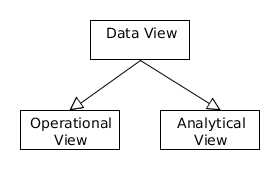
\includegraphics[natwidth=\textwidth]{figures/datamodelling/dataviews.png}
 \centering
 \label{fig:dataviews}
 \caption{Sicht auf Daten. Operational View als Informationsquelle für taktische und Analytical View als Informationsquelle für strategische Entscheidungen.}
\end{figure}

S\o rensen, Fountas und Nash stellen in \cite{jour:Sorensen2010} ein Modell für \textit{Farming Management Information System} kurz FMIS vor. Dies soll als Basis für Planungssysteme wie es aus anderen Branchen als ERP bekannt ist eingesetzt werden. S\o rensen beschreibt dies als drei aufeinander aufbauende Systeme, siehe auch \ref{fig:fmishierarchy}.

\begin{figure}[h]
 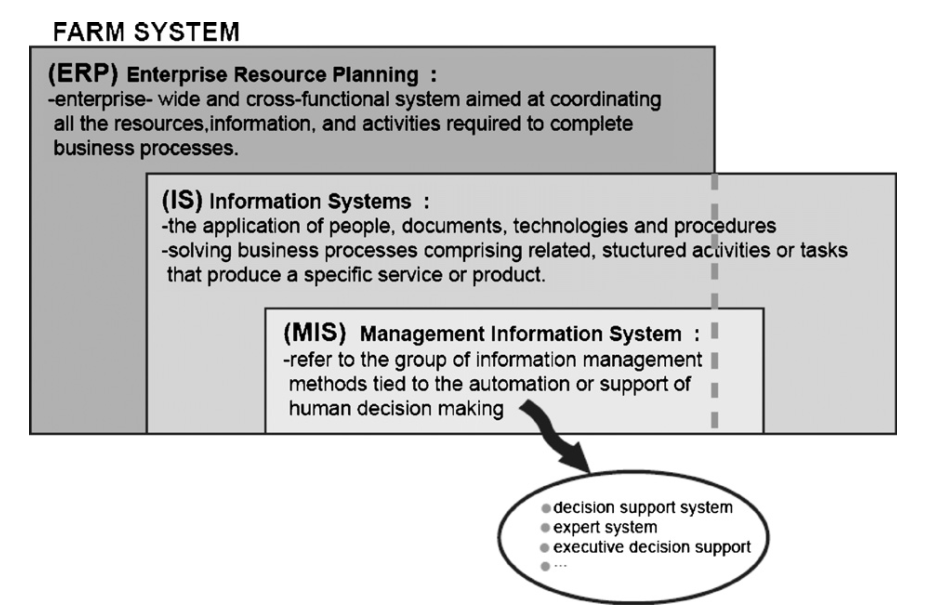
\includegraphics[scale=0.5,natwidth=\textwidth]{figures/datamodelling/sorensen_fmis_2010.png}
 \centering
 \label{fig:fmishierarchy}
 \caption{Konzept eines Management Information Systems.\cite{jour:Sorensen2010}}
\end{figure}

Neben diesen Sichtweisen die für die Entscheidungen im Betrieb wichtig sind, gehen Ruiz-Garcia, Steinberger und Rothmund in \cite{jour:Ruiz-Garcia2010} auf die Modellierung von Daten, Protokollen und Systemen ein, die es erlauben die Verarbeitung der Produkte in allen Schritten der Versorgungskette automatisch überwachen zu lassen. Dies dient dazu, den immer strenger werdenden gesetzlichen Bestimmungen (z.B. der ISO 22005 Standard zur Rückverfolgbarkeit der Lebensmittelbestandteile oder den EU Verordnungen Nr. 178/2002 bzw. Nr. 1935/2004) genügen zu können, ohne die Überprüfungen jedes Lieferanten manuell durchführen zu müssen.

\subsection{Operationale Sicht}
Die operationale Sicht dient dazu Entscheidungen in und für Geschäftsprozesse zu erleichtern bzw. zu ermöglichen. Unternehmerische Geschäftsprozesse werden in \cite{jour:Schulze2007} als Entscheidungen in einem begrenzten Zeitraum beschrieben. Dementsprechend ist es wichtig, dass die operationale Sicht vor allem Daten präsentiert die folgende Bedingungen erfüllen:

\begin{itemize}
	\item Die Daten müssen so aufbereitet werden, dass sie innerhalb der Prozesse verfügbar sind. (\textit{process-orientated data access})
	\item Die Daten müssen aktuell und detailliert sein.
	\item Die Daten müssen Zustände beschreiben. Zustände sollten lt. \cite{jour:Schulze2007} dabei als Menge von Attributen und Relationen zu anderen Zuständen definiert werden.
\end{itemize}

\subsection{Analytische Sicht}
Die analytische Sicht auf die bestehenden Daten leitet sich aus Messungen über einen bestimmten Zeitraum hinweg ab. Als Messungen sind Ergebnisse von bestimmten Berechnungen auf Klassifizierungspfade innerhalb der verfügbaren Datenbasis. In anderen Worten, geht es darum Aggregationen auf Relationen innerhalb von relevanten Ressourcen im Betrieb durchzuführen. Schulze macht dies am Beispiel eines Rinderzuchtsbetriebs für die Milchproduktion deutlich. Dabei werden Informationen über drei Ebenen hinweg aggregiert. So stellt die Sicht auf Ebene der Ställe andere Informationen als auf Ebene der einzelnen Kühe zur Verfügung. Siehe dazu Abbildung \ref{fig:kuehe}. 

\begin{figure}[h]
 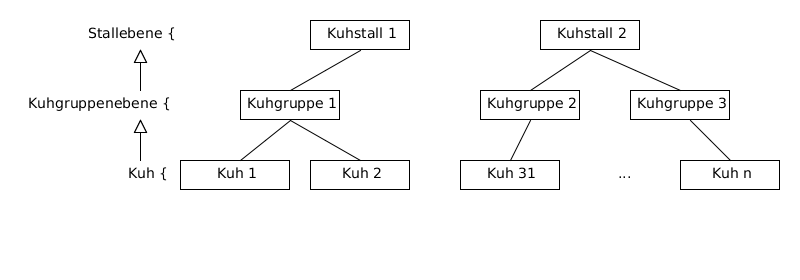
\includegraphics[scale=0.5,natwidth=\textwidth]{figures/datamodelling/kuehe.png}
 \centering
 \label{fig:kuehe}
 \caption{Klassifizierungsschema eines Milcherzeugungsbetriebs.}
\end{figure}

Dadurch wird die analytische Sicht im Unterschied zur operationalen Sicht, durch folgende Eigenschaften definiert:
\begin{itemize}
	\item Die analytische Sicht enthält auch historische Daten.
	\item Die analytische Sicht versucht verschiedene Datenquellen zu integrieren und ein Gesamtbild zu generieren.
	\item Die Daten werden ständig aggregiert und damit wiederverwendet.
\end{itemize}

Multidimensionale Daten können in Form von OLAP-Würfeln visualisiert werden.\ref{fig:kuehe_olap} 

\begin{figure}[h]
 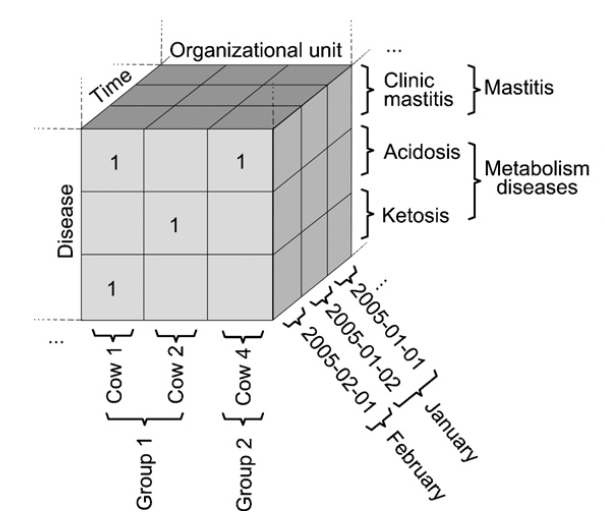
\includegraphics[scale=0.5,natwidth=\textwidth]{figures/datamodelling/kuehe_olap_wuerfel_schulze2007.png}
 \centering
 \label{fig:kuehe_olap}
 \caption{Darstellung der Daten eines Milcherzeugungsbetriebs in Form eines OLAP Würfelns.\cite{jour:Schulze2007}}
\end{figure}

Für die Speicherung und Verarbeitung von solch strukturierten Daten gibt es mehrere Ansätze. Die Daten können entweder getrennt gespeichert und verarbeitet werden in Form der Separierung in OLAP- und OLTP-System, oder auch zusammen geführt werden um die Auswertung auf aktuelleren Daten zu erlauben. Kemper stellt dafür in \cite{jour:Kemper2011} \textit{HyPer} vor.

\section{Entwurf von Datenmodellen}
Das Planen, Entwerfen und Erstellen von Datenmodellen ist ein Prozess, der im Zusammenspiel von Domänenexperten und Datenmodellierungsexperten durchgeführt werden muss. Sowohl S\o rensen wie auch Schulze schlagen dafür einen strukturierten Ansatz vor, der bei der Bestandsaufnahme der Akteure und Ressourcen beginnt und bei der Abbildung der verschiedenen Dimensionen und Relationen endet.\cite{jour:Schulze2007}\cite{jour:Sorensen2010}

Dem oder der Expertin für Datenmodellierung wird dabei nicht nur abverlangt die Relationen und Attribute in den verschiedenen Dimensionen formal abbilden zu können, sondern die Prozesse auch zu identifizieren um sie dann beschreiben zu können. Burkhart, Wolter, Schief, Di Valentin, Werth, Loos und Vaderhaeghen empfehlen dafür eine Ontologie zu entwerfen, stellten aber gleichzeitig fest, dass es noch keine Methode gibt, die völlig zufriedenstellend anleitet.\cite{jour:Burkhart2012} 

Schulz schlägt vor, zur Modellierung der Daten auf ein erweitertes \textit{Entity Relationship Modell}, kurz ER-Modell zurück zu greifen und hat dies auch exemplarisch vorgeführt. 


